% Provenance (never printed): old premiere S material on the oceanic lithosphere
% (ophiolite-type layering, peridotite and gabbro, partial melting by decompression
% at the ridge, hydrothermalism, cooling and subsidence of the lithosphere with
% age); see sources/book2/PROVENANCE.md. Melting from figdata/grade-11/
% ridge_melting.py (adiabat and Hirschmann solidus), depth against age from
% depth_age.py (ETOPO1 and the Seton 2020 age grid). Partial melting is re-founded
% in Year 2 (mantle-melting); fault is Book 1's (g7), normal fault is defined here.
\chapter{As dorsais oceânicas e a litosfera oceânica}\label{ch:g11:ocean-ridges}

Em fevereiro de 1977, um trenó com câmeras rebocado a 2500 metros de
profundidade sobre o Rifte de Galápagos, no Pacífico oriental, fotografava
quadro após quadro a lava negra e nua da dorsal. Então o seu termômetro
registrou uma pequena alta na temperatura da água, e nas fotografias a lava
apareceu coberta de centenas de mariscos brancos. Poucos dias depois, o
submersível \emph{Alvin} levou dois geólogos até o local: uma água morna e
tremulante saía das fendas da lava, e em volta viviam mariscos do tamanho de
um antebraço, mexilhões e caranguejos brancos; num mergulho posterior,
vermes tubulares de pontas vermelhas. Ninguém esperava vida ali, e por isso
não havia nenhum biólogo a bordo. Este capítulo explica o que os geólogos
tinham encontrado: como o fundo do oceano é feito nas dorsais, por que ele é
quente ali, e o que acontece com ele à medida que se afasta.
% ledger: whoi:alvin-1977

\begin{recall}
Nas dorsais, um novo fundo oceânico é feito e se afasta dos dois lados, de
modo que a sua idade cresce com a distância ao eixo; as dorsais formam um
sistema de cerca de \qty{65000}{km} de comprimento, com um vale de rifte ao
longo das dorsais lentas e uma crista suave ao longo das rápidas
(\cref{ch:g11:drift-to-spreading}). As placas se afastam através de uma
dorsal a alguns centímetros por ano, mais depressa através da Dorsal do
Pacífico Oriental do que através da Dorsal Mesoatlântica
(\cref{ch:g11:plate-motions}). A \omterm{def:g11:lithosphere-asthenosphere:lithosphere}{litosfera} é a camada externa rígida, e a
\omterm{def:g11:lithosphere-asthenosphere:lithosphere}{astenosfera} abaixo dela escoa; a temperatura da \omterm{def:g11:lithosphere-asthenosphere:lithosphere}{astenosfera} sobe apenas
cerca de \qty{0.45}{\celsius} por quilômetro de profundidade, e a
temperatura de fusão da rocha do manto sobe com a profundidade
(\cref{ch:g11:lithosphere-asthenosphere}). O magma é rocha fundida abaixo da
superfície, o basalto a rocha escura que a lava forma ao esfriar, e uma
falha uma ruptura ao longo da qual as rochas se deslocaram (Livro 1, 6º e
7º anos).
\end{recall}
% ledger: noaa:ridge, katsura10:adiabat, hirschmann:solidus

\section{A litosfera oceânica}

Duas rochas raras na superfície dos continentes formam a maior parte da
\omterm{def:g11:ocean-ridges:oceanic-lithosphere}{litosfera oceânica}.

\begin{definition}[Peridotito]\label{def:g11:ocean-ridges:peridotite}
O \emph{peridotito}\index{peridotito} é uma rocha escura, de grão grosso,
feita principalmente do mineral olivina, com um pouco de piroxênio. Ele é
geralmente verde e denso. Acredita-se que grande parte do manto da Terra
seja feita de peridotito.
\end{definition}

\begin{definition}[Gabro]\label{def:g11:ocean-ridges:gabbro}
O \emph{gabro}\index{gabro} é uma rocha ígnea escura, de grão grosso, feita
principalmente de feldspato plagioclásio e piroxênio. Ele tem a mesma
composição que o basalto, mas cristalizou lentamente, no fundo do subsolo,
o que deu aos seus cristais tempo para crescer. É a rocha mais abundante da
\omterm{def:g11:ocean-ridges:oceanic-lithosphere}{crosta oceânica} profunda.
\end{definition}
% ledger: geo:peridotite, geo:gabbro

Os minerais citados aqui, olivina, piroxênio e feldspato, são descritos no
\cref{ch:g11:minerals}.

\begin{omfigure}
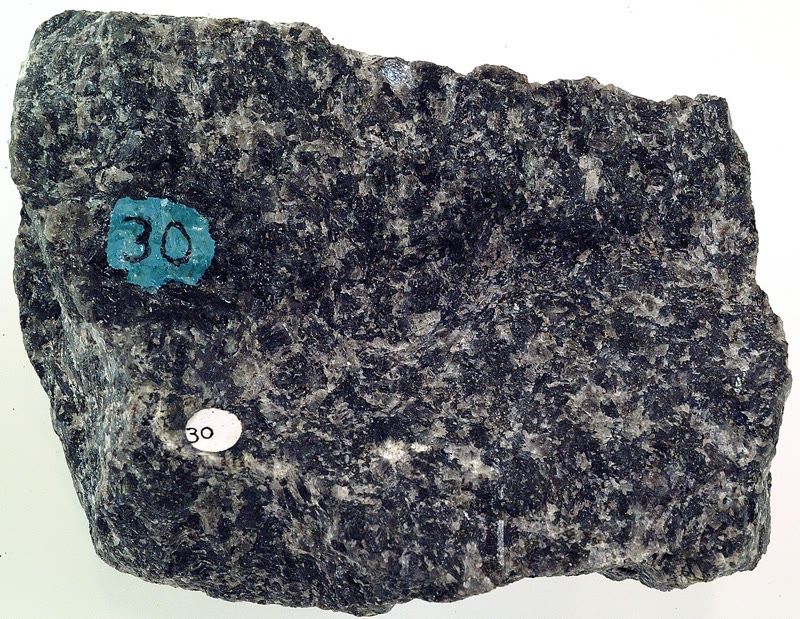
\includegraphics[height=4.2cm]{images/book2/g11-geodil-gabbro.jpg}\hspace{0.03\linewidth}%
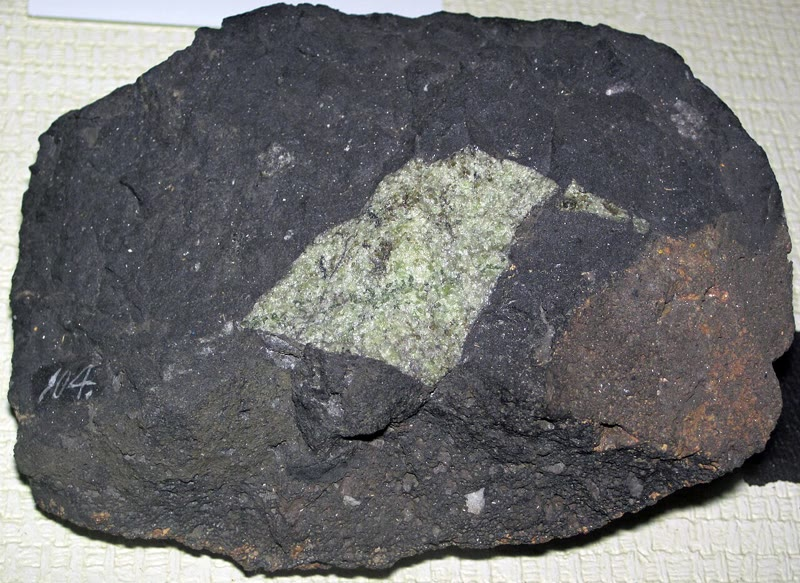
\includegraphics[height=4.2cm]{images/book2/g11-stjohn-peridotite.jpg}

{\small À esquerda: \omterm{def:g11:ocean-ridges:gabbro}{gabro}, com \qty{9}{cm} de largura, com cristais escuros
de piroxênio e claros de feldspato grandes o bastante para serem vistos;
fotografia Darla Sondrol (CC0). À direita: um pedaço de \omterm{def:g11:ocean-ridges:peridotite}{peridotito} verde do
manto, trazido para cima dentro da lava basáltica negra de um vulcão no
Arizona; fotografia James St.~John (CC~BY~2.0).}
\end{omfigure}
% ledger: photo:g11-gabbro, photo:g11-peridotite

\begin{definition}[Crosta oceânica; litosfera oceânica]\label{def:g11:ocean-ridges:oceanic-lithosphere}
A \emph{crosta oceânica}\index{crosta oceanica@crosta oceânica} é a crosta do
fundo do oceano: cerca de \qty{7}{km} de basalto e de \omterm{def:g11:ocean-ridges:gabbro}{gabro}, feitos nas
dorsais. A \emph{litosfera oceânica}\index{litosfera oceanica@litosfera oceânica}
é a crosta oceânica junto com o \omterm{def:g11:ocean-ridges:peridotite}{peridotito} rígido do manto mais alto, abaixo
dela.
\end{definition}

Os levantamentos sísmicos em todos os oceanos dão à \omterm{def:g11:ocean-ridges:oceanic-lithosphere}{crosta oceânica} uma
espessura média de \qty{7.1}{km}, com variação de \qty{0.8}{km} para mais
ou para menos, longe das zonas de fratura e dos pontos quentes. As suas
camadas são conhecidas por perfurações profundas e por fatias de fundo
oceânico antigo empurradas sobre os continentes. Em 2005, um navio-sonda
terminou um furo de \qty{1507}{m} de profundidade numa crosta de 15 milhões
de anos do Pacífico oriental, o primeiro a passar das lavas, através dos
diques, até os \omterm{def:g11:ocean-ridges:gabbro}{gabros}:
% ledger: white92:crust, iodp1256:section, geo:peridotite

\begin{itemize}
  \item no topo, uma fina cobertura de \emph{sedimentos}, ausente no eixo da
        dorsal e mais espessa no fundo mais antigo;
  \item mais de \qty{800}{m} de \emph{lavas basálticas}, que irromperam no
        fundo do mar em lençóis e em \emph{almofadas}, tubos e bolhas
        arredondados de lava com uma pele vítrea;
  \item o \emph{complexo de diques}, \qty{346}{m} neste furo: centenas de
        lâminas verticais de basalto, cada uma a fenda congelada pela qual o
        magma subiu até uma erupção, lado a lado como as páginas de um livro;
  \item o \emph{\omterm{def:g11:ocean-ridges:gabbro}{gabro}}, alcançado a \qty{1407}{m} abaixo do fundo do mar, o
        magma que cristalizou lentamente abaixo dos diques, até o \omterm{def:g11:seismic-structure:moho}{Moho};
  \item abaixo do \omterm{def:g11:seismic-structure:moho}{Moho}, o \emph{\omterm{def:g11:ocean-ridges:peridotite}{peridotito}} do manto.
\end{itemize}
% ledger: iodp1256:section, geo:basalt-ridges, geo:gabbro

\begin{omfigure}
\begin{tikzpicture}[x=1cm, y=-0.55cm, font=\footnotesize]
% to scale in depth: lavas 0.8 km, dykes 0.35 km (iodp1256:section), crust 7.1 km (white92:crust)
  \fill[omLithAlluv] (0,-0.25) rectangle (2.4,0);
  \fill[lith basalt] (0,0) rectangle (2.4,0.8);
  \fill[omLithBasalt!60] (0,0.8) rectangle (2.4,1.15);
  \foreach \x in {0.15,0.35,...,2.3} \draw[black!55, line width=0.3pt] (\x,0.8) -- (\x,1.15);
  \fill[lith gabbro] (0,1.15) rectangle (2.4,7.1);
  \fill[lith peridotite] (0,7.1) rectangle (2.4,9.0);
  \draw (0,-0.25) rectangle (2.4,9.0);
  \draw[line width=0.9pt] (0,7.1) -- (2.4,7.1);
  \foreach \d in {0,2,4,6,8} {\draw (-0.1,\d) -- (0,\d); \node[anchor=east] at (-0.1,\d) {\d};}
  \node[rotate=90, anchor=south] at (-0.75,4.5) {profundidade abaixo do fundo do mar (\unit{km})};
  \draw[black!60] (2.4,-0.13) -- (2.7,-1.0) -- (2.85,-1.0);
  \node[anchor=west] at (2.85,-1.0) {sedimentos};
  \draw[black!60] (2.4,0.4) -- (2.7,0.25) -- (2.85,0.25);
  \node[anchor=west] at (2.85,0.25) {lavas: almofadas e derrames em lençol};
  \draw[black!60] (2.4,0.98) -- (2.7,1.6) -- (2.85,1.6);
  \node[anchor=west] at (2.85,1.6) {complexo de diques};
  \node[anchor=west] at (2.55,4.1) {gabro};
  \node[anchor=west] at (2.55,7.1) {Moho};
  \node[anchor=west] at (2.55,8.05) {peridotito do manto};
  \draw[decorate, decoration={brace, amplitude=5pt}] (7.9,0) -- (7.9,7.1)
    node[midway, right=7pt, align=left] {crosta oceânica\\cerca de \qty{7}{km}};
\end{tikzpicture}

{\small As camadas da \omterm{def:g11:ocean-ridges:oceanic-lithosphere}{crosta oceânica}, com as profundidades em escala. As
espessuras das lavas e dos diques são as do furo profundo perfurado no
Pacífico oriental; a espessura total é a média dos levantamentos sísmicos. A
cobertura de sedimentos fica mais espessa com a idade do fundo.}
\end{omfigure}
% ledger: iodp1256:section, white92:crust

\begin{omfigure}
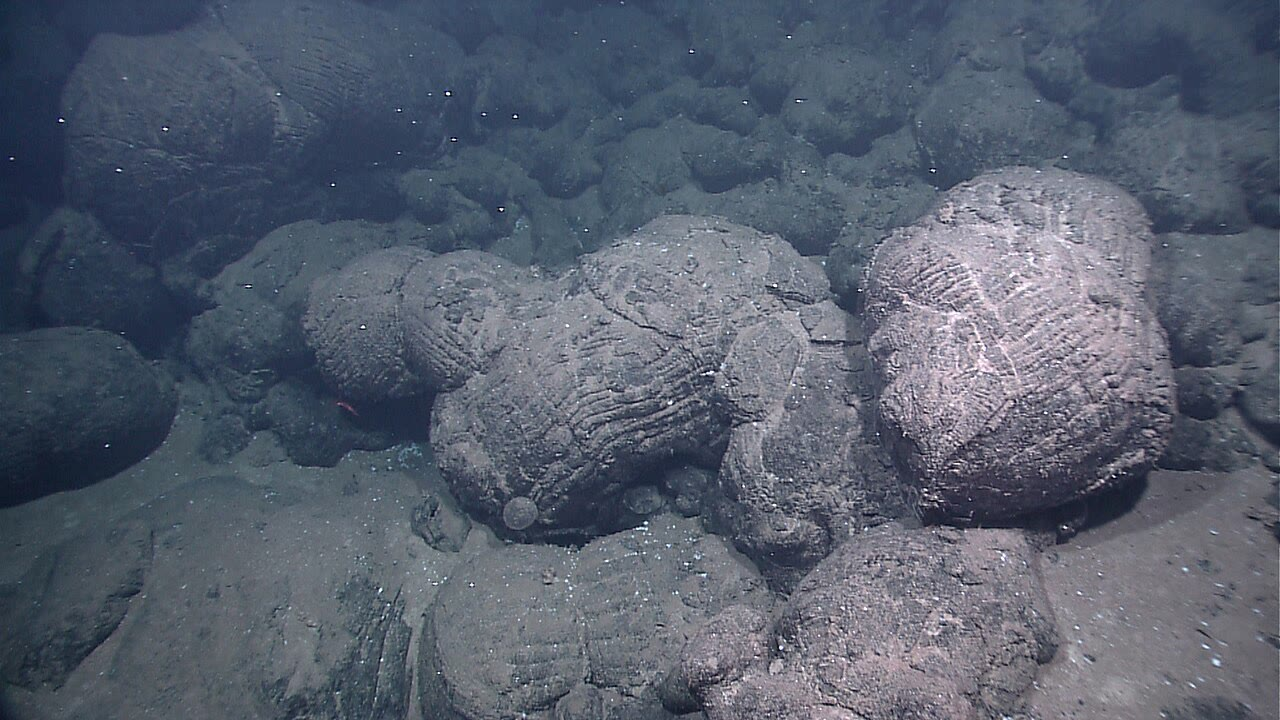
\includegraphics[width=0.8\linewidth]{images/book2/g11-noaa-pillow-lava.jpg}

{\small Lava em almofada no Rifte de Galápagos, a cerca de 2500 metros de
profundidade, fotografada por um veículo operado remotamente em 2011. Cada
almofada é uma língua de lava que congelou por fora no instante em que
encontrou a água fria do mar. Fotografia: NOAA Okeanos Explorer Program
(domínio público).}
\end{omfigure}
% ledger: photo:g11-pillow-lava, whoi:alvin-1977 (depth of the rift floor)

\section{Fundir sem aquecer}

O manto sob uma dorsal é \omterm{def:g11:ocean-ridges:peridotite}{peridotito} sólido, como em qualquer outro lugar. No
entanto, \qty{7}{km} de basalto e de \omterm{def:g11:ocean-ridges:gabbro}{gabro}, uma rocha fundida que
solidificou, saem dele. De onde vem o material fundido?

\begin{definition}[Fusão parcial; fusão por descompressão]\label{def:g11:ocean-ridges:partial-melting}
A \emph{fusão parcial}\index{fusao parcial@fusão parcial} é a fusão de apenas
uma parte de uma rocha: alguns dos seus minerais, ou alguns dos seus
componentes, fundem, enquanto o resto continua sólido.
A \emph{fusão por descompressão}\index{fusao por descompressao@fusão por descompressão} é a fusão parcial de uma rocha que sobe, e por isso fica cada vez
menos comprimida, sem ser aquecida.
\end{definition}

Quando duas placas se afastam, a \omterm{def:g11:lithosphere-asthenosphere:lithosphere}{astenosfera} sobe sob a dorsal para
preencher o vão. Ela sobe depressa demais para perder muito calor, de modo
que a sua temperatura cai apenas cerca de \qty{0.45}{\celsius} por
quilômetro na subida. A sua temperatura de fusão, que depende da pressão,
cai muito mais depressa: cerca de \qty{3.9}{\celsius} por quilômetro a uma
profundidade de \qty{50}{km}. A certa profundidade, a rocha que sobe atinge
a sua temperatura de fusão e começa a fundir, embora nenhum calor tenha sido
acrescentado.
% ledger: katsura10:adiabat, hirschmann:solidus, white92:crust; computed in
% figdata/grade-11/ridge_melting.py (solidus_slope_50km 3.89)

\begin{method}[Onde o manto que sobe funde?]\label{met:g11:ocean-ridges:melting}
\begin{enumerate}
  \item Escreva a temperatura da rocha que sobe em cada profundidade: a sua
        temperatura potencial (a temperatura que ela teria na superfície)
        mais \qty{0.45}{\celsius} por quilômetro de profundidade.
  \item Escreva a temperatura de fusão da rocha em cada profundidade, a
        partir da pressão nessa profundidade.
  \item Encontre a profundidade em que as duas são iguais. Mais fundo, a
        rocha é sólida; mais acima, ela está parcialmente fundida.
\end{enumerate}
\end{method}

\begin{omfigure}
\begin{tikzpicture}
\begin{axis}[omrecord, omdepth, width=0.72\linewidth, height=6.4cm, xmin=1100, xmax=1700, ymin=0, ymax=150,
  xlabel={temperatura (\unit{\celsius})}, ylabel={profundidade (\unit{km})},
  xticklabel style={/pgf/number format/set thousands separator={}}, clip=true]
% computed in figdata/grade-11/ridge_melting.py; ledger: katsura10:adiabat, hirschmann:solidus, data:prem
\addplot[omProp, line width=1.0pt] table[x=solidus, y=z] {figdata/out/grade-11-ridge_melting-curves.dat};
\addplot[omDef, line width=1.0pt] table[x=ad1300, y=z] {figdata/out/grade-11-ridge_melting-curves.dat};
\addplot[omDef, densely dashed, line width=0.9pt] table[x=ad1400, y=z] {figdata/out/grade-11-ridge_melting-curves.dat};
\addplot[only marks, mark=*, mark size=1.8pt, black] coordinates {(1324.3,54.1) (1438.3,85.0)};
\node[font=\scriptsize, anchor=east, align=right] at (axis cs:1316,62) {início da fusão,\\a \qty{54}{km}};
\node[font=\scriptsize, anchor=east] at (axis cs:1432,89) {\qty{85}{km}};
\node[font=\scriptsize, text=omProp, anchor=west, align=left] at (axis cs:1560,40) {temperatura\\de fusão};
\node[font=\scriptsize, text=omDef, anchor=east, align=right] at (axis cs:1318,128) {manto que sobe,\\$T_p = \qty{1300}{\celsius}$};
\node[font=\scriptsize, text=omDef, anchor=west, align=left] at (axis cs:1476,140) {$T_p = \qty{1400}{\celsius}$};
\end{axis}
\end{tikzpicture}

{\small A temperatura da rocha do manto que sobe sob uma dorsal (azul) e a
sua temperatura de fusão (laranja), em função da profundidade. A rocha com
temperatura potencial de \qty{1300}{\celsius} começa a fundir a
\qty{54}{km} de profundidade; a rocha \qty{100}{\celsius} mais quente
(tracejado), já a \qty{85}{km}. Temperatura de fusão do \omterm{def:g11:ocean-ridges:peridotite}{peridotito} seco
obtida em experimentos (Hirschmann, 2000).}
\end{omfigure}
% values: onset_1300_km 54.1, onset_1400_km 85.0, t_onset_1300 1324 (ridge_melting.py)

\begin{example}[A profundidade da fusão]\label{ex:g11:ocean-ridges:onset}
Para um manto de temperatura potencial \qty{1300}{\celsius}, a rocha que
sobe está a $1300 + 0.45 \times 54 \approx \qty{1324}{\celsius}$ quando chega
a \qty{54}{km}, exatamente a sua temperatura de fusão nessa profundidade: a
fusão começa a cerca de \qty{54}{km} de profundidade. Acima dessa
profundidade, a rocha continua fundindo enquanto sobe.
\end{example}

Só uma pequena fração do \omterm{def:g11:ocean-ridges:peridotite}{peridotito} funde, e o material fundido não é
\omterm{def:g11:ocean-ridges:peridotite}{peridotito}: é basalto. Os líquidos basálticos se reúnem de toda a região de
fusão, que vai da profundidade de início até a base da crosta; mais leves
que a rocha sólida em volta, eles sobem até o eixo da dorsal. Ali, parte do
magma irrompe como lava, parte congela como diques nas fendas pelas quais
subiu, e parte cristaliza lentamente mais abaixo como \omterm{def:g11:ocean-ridges:gabbro}{gabro}. O \omterm{def:g11:ocean-ridges:peridotite}{peridotito}
sólido que fica para trás, empobrecido do seu basalto, torna-se a parte
mantélica da \omterm{def:g11:ocean-ridges:oceanic-lithosphere}{litosfera oceânica}.
% ledger: asimow01:morb, geo:basalt-ridges, white92:crust

Onde uma dorsal atravessa uma região de manto mais quente, em volta de um
ponto quente, a fusão começa mais fundo, uma coluna de rocha mais longa
funde e mais basalto é produzido: ali a crosta tem cerca de \qty{10}{km} de
espessura em vez de 7. Ao contrário, sob dorsais muito lentas, o manto que
sobe tem tempo de perder calor, funde menos e produz uma crosta
excepcionalmente fina.
% ledger: white92:crust

\begin{omfigure}
\begin{tikzpicture}[font=\footnotesize]
  % schematic section across a ridge axis, not to scale
  \fill[omSea!45] (-6,0) rectangle (6,1.2);
  \fill[lith basalt] (-6,0) -- (-0.25,0) -- (-0.25,-0.35) -- (-6,-0.6) -- cycle;
  \fill[lith basalt] (6,0) -- (0.25,0) -- (0.25,-0.35) -- (6,-0.6) -- cycle;
  \fill[lith gabbro] (-6,-0.6) -- (-0.25,-0.35) -- (-0.25,-1.4) -- (-6,-1.6) -- cycle;
  \fill[lith gabbro] (6,-0.6) -- (0.25,-0.35) -- (0.25,-1.4) -- (6,-1.6) -- cycle;
  \fill[lith basalt] (-0.3,0) rectangle (0.3,-0.35);
  \fill[lith gabbro] (-0.3,-0.35) rectangle (0.3,-1.45);
  \fill[omProp!70] (-0.8,-0.75) .. controls (-0.4,-0.55) and (0.4,-0.55) .. (0.8,-0.75)
     .. controls (0.4,-0.95) and (-0.4,-0.95) .. (-0.8,-0.75);
  \fill[omProp!70] (-0.12,0) rectangle (0.12,-0.62);
  \fill[lith peridotite] (-6,-1.6) -- (-0.25,-1.4) -- (0.25,-1.4) -- (6,-1.6) -- (6,-5) -- (-6,-5) -- cycle;
  % melting region
  \fill[omProp!35] (-3.2,-1.5) -- (0,-4.0) -- (3.2,-1.5) -- cycle;
  \node[align=center] at (0,-2.95) {região de fusão};
  % isotherms deepening away from the axis
  \draw[omDef!70!black, densely dashed] (-6,-2.6) .. controls (-2.5,-2.0) and (-1,-1.1) .. (0,-1.0) .. controls (1,-1.1) and (2.5,-2.0) .. (6,-2.6);
  \draw[omDef!70!black, densely dashed] (-6,-4.2) .. controls (-3,-3.6) and (-1.2,-2.0) .. (0,-1.9) .. controls (1.2,-2.0) and (3,-3.6) .. (6,-4.2);
  \node[text=omDef!70!black, anchor=west] at (6.05,-2.6) {\qty{800}{\celsius}};
  \node[text=omDef!70!black, anchor=west] at (6.05,-4.2) {\qty{1200}{\celsius}};
  % flow arrows
  \draw[-{Stealth[length=5pt]}, line width=0.9pt] (0,-4.9) -- (0,-4.2);
  \draw[-{Stealth[length=5pt]}, line width=0.9pt] (-1.2,-4.8) .. controls (-1.0,-3.8) and (-2.2,-3.2) .. (-3.6,-3.2);
  \draw[-{Stealth[length=5pt]}, line width=0.9pt] (1.2,-4.8) .. controls (1.0,-3.8) and (2.2,-3.2) .. (3.6,-3.2);
  \draw[-{Stealth[length=5pt]}, line width=1.1pt] (-2,0.6) -- (-4,0.6);
  \draw[-{Stealth[length=5pt]}, line width=1.1pt] (2,0.6) -- (4,0.6);
  \node[anchor=south] at (-3,0.65) {placa};
  \node[anchor=south] at (3,0.65) {placa};
  \node[anchor=west] at (1.0,-0.8) {lente de magma};
  \node[anchor=east] at (-6.05,-0.3) {lavas};
  \node[anchor=east] at (-6.05,-1.1) {gabro};
  \node[anchor=east] at (-6.05,-3.3) {manto};
  \node[anchor=north] at (0,-5.05) {o manto sobe e funde};
\end{tikzpicture}

{\small Um corte através do eixo de uma dorsal (um desenho, fora de escala).
O manto sobe sob o eixo e funde em parte; o material fundido se reúne numa
lente de magma sob o eixo e constrói a crosta, que as placas levam embora
dos dois lados. As linhas de mesma temperatura (tracejadas) ficam perto da
superfície no eixo e cada vez mais fundo longe dele: a \omterm{def:g11:lithosphere-asthenosphere:lithosphere}{litosfera} fica mais
espessa à medida que esfria.}
\end{omfigure}

\section{Dorsais rápidas e lentas}

As dorsais se abrem a velocidades muito diferentes. Calculadas a partir dos
polos de rotação do \cref{ch:g11:plate-motions}, a Dorsal do Pacífico
Oriental a \ang{30} Sul se abre a \qty{14.6}{cm} por ano, e a Dorsal
Mesoatlântica na mesma latitude a \qty{3.3}{cm} por ano. A forma do eixo não
é a mesma.
% ledger: nnr56:poles (computed in plate_velocities.py: epr30s_speed 145.8, atl30s_speed 32.7)

Ao longo das dorsais lentas, o eixo é um vale de 1 a \qty{2}{km} de
profundidade e de 20 a \qty{30}{km} de largura. Chega muito pouco magma ao
eixo para preencher o vão continuamente: a \omterm{def:g11:lithosphere-asthenosphere:lithosphere}{litosfera} fria e frágil é
estirada e se rompe ao longo de falhas.

\begin{definition}[Falha normal]\label{def:g11:ocean-ridges:normal-fault}
Uma \emph{falha normal}\index{falha normal} é uma falha inclinada ao longo
da qual o bloco acima do plano de falha desceu em relação ao bloco abaixo
dele. As falhas normais se formam onde a crosta é estirada.
\end{definition}

O vale de uma dorsal lenta é um bloco que desceu entre \omterm{def:g11:ocean-ridges:normal-fault}{falhas normais}
voltadas uma para a outra; quase todas mergulham em direção ao eixo. Um
bloco rebaixado assim entre \omterm{def:g11:ocean-ridges:normal-fault}{falhas normais} se chama \emph{graben}.
% ledger: buck05:valley, usgs:normal-fault

Ao longo das dorsais rápidas, o magma chega com frequência suficiente para
preencher o vão. O eixo é um alto suave e pouco inclinado, sobre uma lente
de magma que fica abaixo dele.
% ledger: buck05:valley, noaa:ridge

\begin{omfigure}
\begin{tikzpicture}[font=\footnotesize, x=0.24cm, y=0.9cm]
  % slow ridge: axial valley between normal faults (not to scale, vertical exaggeration)
  \begin{scope}
    \fill[omSea!45] (-15,-0.7) rectangle (15,1.6);
    \fill[lith basalt] (-15,0.9) -- (-9,0.9) -- (-8.5,0.2) -- (-6,0.2) -- (-5.5,-0.6) -- (5.5,-0.6)
      -- (6,0.2) -- (8.5,0.2) -- (9,0.9) -- (15,0.9) -- (15,-2.2) -- (-15,-2.2) -- cycle;
    \draw[black!70] (-15,0.9) -- (-9,0.9) -- (-8.5,0.2) -- (-6,0.2) -- (-5.5,-0.6) -- (5.5,-0.6)
      -- (6,0.2) -- (8.5,0.2) -- (9,0.9) -- (15,0.9);
    \draw[fault] (-9,0.9) -- (-7.4,-2.2);
    \draw[fault] (-6,0.2) -- (-4.6,-2.2);
    \draw[fault] (9,0.9) -- (7.4,-2.2);
    \draw[fault] (6,0.2) -- (4.6,-2.2);
    % slip arrows on the hanging walls (the axis side of each fault): down along the fault
    \foreach \x/\y/\s in {-7.9/-0.5/1, -5.0/-1.3/1, 7.9/-0.5/-1, 5.0/-1.3/-1} {
      \draw[-{Stealth[length=3pt]}, omProp, line width=0.8pt] (\x+0.9*\s,\y+0.45) -- ++(0.3*\s,-0.6);
    }
    \draw[-{Stealth[length=5pt]}, line width=1pt] (-11,1.25) -- (-14,1.25);
    \draw[-{Stealth[length=5pt]}, line width=1pt] (11,1.25) -- (14,1.25);
    \node at (0,-0.25) {vale axial};
    \node[anchor=north, align=center] at (0,-2.25) {dorsal lenta: um vale\\entre falhas normais};
  \end{scope}
  % fast ridge
  \begin{scope}[xshift=8.2cm]
    \fill[omSea!45] (-15,0) rectangle (15,1.6);
    \fill[lith basalt] (-15,0.3) .. controls (-6,0.4) and (-2,0.9) .. (0,0.95) .. controls (2,0.9) and (6,0.4) .. (15,0.3)
      -- (15,-2.2) -- (-15,-2.2) -- cycle;
    \fill[omProp!75] (-2.5,-0.9) .. controls (-1,-0.7) and (1,-0.7) .. (2.5,-0.9) .. controls (1,-1.1) and (-1,-1.1) .. (-2.5,-0.9);
    \draw[black!70] (-15,0.3) .. controls (-6,0.4) and (-2,0.9) .. (0,0.95) .. controls (2,0.9) and (6,0.4) .. (15,0.3);
    \node[anchor=north] at (0,-1.25) {lente de magma};
    \draw[-{Stealth[length=5pt]}, line width=1pt] (-8,1.25) -- (-14,1.25);
    \draw[-{Stealth[length=5pt]}, line width=1pt] (8,1.25) -- (14,1.25);
    \node at (0,1.3) {alto axial};
    \node[anchor=north, align=center] at (0,-2.25) {dorsal rápida: um alto suave\\sobre uma lente de magma};
  \end{scope}
\end{tikzpicture}

{\small Cortes através de uma dorsal lenta e de uma dorsal rápida (desenhos,
fora de escala; a altura está exagerada). À esquerda: o vale axial de uma
dorsal lenta, de 1 a \qty{2}{km} de profundidade, desceu entre \omterm{def:g11:ocean-ridges:normal-fault}{falhas
normais} que mergulham em direção ao eixo (setas laranja: os blocos acima das
falhas deslizam para baixo). À direita: uma dorsal rápida se eleva
suavemente acima de uma lente de magma.}
\end{omfigure}
% ledger: buck05:valley

\begin{example}[Uma dorsal lenta e uma dorsal rápida]\label{ex:g11:ocean-ridges:rates}
Em um milhão de anos, a Dorsal do Pacífico Oriental a \ang{30} Sul produz
$\qty{14.6}{cm/yr} \times 10^6\ \text{anos} = \qty{146}{km}$ de novo fundo
oceânico, \qty{73}{km} de cada lado; a Dorsal Mesoatlântica na mesma
latitude produz \qty{33}{km}, \qty{16.5}{km} de cada lado. O furo profundo
do Pacífico oriental entrou numa crosta feita a mais de \qty{20}{cm} por
ano, uma das expansões mais rápidas já registradas.
\end{example}
% ledger: nnr56:poles (computed), iodp1256:section

\section{As fontes hidrotermais}

A crosta jovem no eixo é quente, e é quebrada por fendas. A água do mar
encontra um caminho para dentro.

\begin{definition}[Circulação hidrotermal; fumarola negra]\label{def:g11:ocean-ridges:hydrothermal}
A \emph{circulação hidrotermal}\index{circulacao hidrotermal@circulação hidrotermal} é o
escoamento da água do mar para baixo pelas fendas da \omterm{def:g11:ocean-ridges:oceanic-lithosphere}{crosta oceânica} quente,
onde ela é aquecida pelo magma abaixo e reage com a rocha, e de volta para
cima até o fundo do mar, onde sai pelas \emph{fontes hidrotermais}. Uma
\emph{fumarola negra}\index{fumarola negra} é uma fonte da qual jorra água
muito quente carregada de metais dissolvidos; ao encontrar a água fria do
mar, sulfetos de ferro e outros minerais precipitam como uma nuvem negra, e
constroem uma chaminé em volta da fonte.
\end{definition}
% ledger: whoi:vents

A água de uma \omterm{def:g11:ocean-ridges:hydrothermal}{fumarola negra} sai tipicamente da sua chaminé a cerca de
\qty{350}{\celsius}, e as águas das fontes podem chegar a
\qty{400}{\celsius}. Elas não fervem, porque dois quilômetros e meio de água
pesam sobre elas. As chaminés podem crescer mais de \qty{10}{m} de altura.
Em volta das fontes, bactérias tiram a sua energia do sulfeto de hidrogênio
da água da fonte, e alimentam vermes tubulares, camarões e mexilhões: os
mariscos do Rifte de Galápagos viviam disso. A maioria das fontes fica ao
longo das dorsais meso-oceânicas.
% ledger: whoi:vents, whoi:alvin-1977

\begin{omfigure}
\begin{minipage}[c]{0.6\linewidth}\centering
\begin{tikzpicture}[font=\scriptsize, x=0.8cm, y=0.62cm]
  \fill[omSea!45] (0,0) rectangle (10,3);
  \fill[lith basalt] (0,0) rectangle (10,-4);
  \fill[omProp!70] (2,-4.6) .. controls (4,-4.0) and (6,-4.0) .. (8,-4.6) -- (8,-5) -- (2,-5) -- cycle;
  \node at (5,-4.7) {magma};
  \fill[black!75] (4.7,0) -- (4.85,1.6) -- (5.15,1.6) -- (5.3,0) -- cycle;
  \fill[black!45, opacity=0.8] (5,1.7) circle (0.35) (5.2,2.2) circle (0.45) (4.9,2.7) circle (0.4);
  \draw[-{Stealth[length=4pt]}, omDef, line width=0.9pt] (1,0) .. controls (1,-2.5) and (2.5,-3.6) .. (4.2,-3.5);
  \draw[-{Stealth[length=4pt]}, omDef, line width=0.9pt] (9,0) .. controls (9,-2.5) and (7.5,-3.6) .. (5.8,-3.5);
  \draw[-{Stealth[length=4pt]}, omProp, line width=1.1pt] (5,-3.3) -- (5,-0.1);
  \node[align=center, text=omDef!80!black] at (1.6,1.0) {entra água\\fria do mar};
  \node[align=left, anchor=west] at (5.6,1.4) {fumarola negra,\\cerca de \qty{350}{\celsius}};
  \node[align=left, anchor=west, text=omProp!80!black, fill=white, fill opacity=0.85, text opacity=1, inner sep=1.5pt] at (5.3,-1.8) {aquecida,\\sobe};
\end{tikzpicture}
\end{minipage}\hfill
\begin{minipage}[c]{0.3\linewidth}\centering
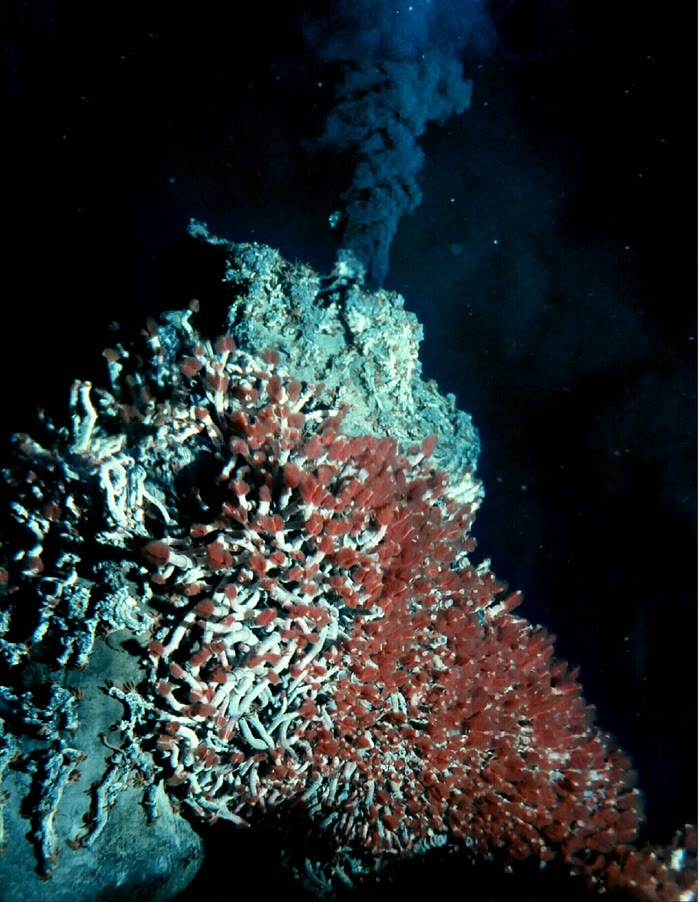
\includegraphics[width=\linewidth]{images/book2/g11-noaa-black-smoker.jpg}
\end{minipage}

{\small À esquerda: a \omterm{def:g11:ocean-ridges:hydrothermal}{circulação hidrotermal} no eixo de uma dorsal (um
desenho, fora de escala). À direita: uma \omterm{def:g11:ocean-ridges:hydrothermal}{fumarola negra} na Dorsal de Juan de
Fuca, com a chaminé coberta de vermes tubulares de brânquias vermelhas;
fotografia University of Washington e NOAA (domínio público).}
\end{omfigure}
% ledger: whoi:vents, photo:g11-black-smoker

\begin{history}[O \emph{Alvin} no Rifte de Galápagos, 1977]
A expedição, financiada pela National Science Foundation, começou em
8~de fevereiro de 1977 a bordo do navio de pesquisa \emph{Knorr}. O trenó de
câmeras ANGUS, rebocado a \qty{2500}{m} de profundidade sobre o rifte,
registrou uma alta na temperatura da água, e nos mesmos quadros as suas
fotografias mostraram centenas de mariscos brancos e conchas marrons de
mexilhões sobre a lava. No mergulho 713 do \emph{Alvin}, os geólogos Jack
Corliss e Tjeerd van Andel encontraram água a \qty{8}{\celsius} saindo
tremulante das fendas, depois até \qty{17}{\celsius}, enquanto a água
profunda em volta estava a \qty{2}{\celsius}; mariscos brancos de até
\qty{30}{cm} de comprimento cobriam uma área de cerca de \qty{50}{m} de
largura. Não havia nenhum biólogo a bordo: a expedição tinha vindo pela água
quente, e encontrou uma comunidade de animais que ninguém tinha imaginado.
\end{history}
% ledger: whoi:alvin-1977

\section{Esfriar, engrossar, afundar}

À medida que se afasta do eixo, a \omterm{def:g11:lithosphere-asthenosphere:lithosphere}{litosfera} esfria por cima, através do
oceano frio acima dela. A camada esfriada fica mais espessa com o tempo: a
\omterm{def:g11:lithosphere-asthenosphere:lithosphere}{litosfera} engrossa, de alguns quilômetros no eixo até cerca de cem
quilômetros no fundo antigo. A rocha esfriada se contrai e fica mais densa,
de modo que a \omterm{def:g11:lithosphere-asthenosphere:lithosphere}{litosfera} flutua mais baixo sobre a \omterm{def:g11:lithosphere-asthenosphere:lithosphere}{astenosfera} (\omterm{def:g11:lithosphere-asthenosphere:isostasy}{isostasia},
\cref{ch:g11:lithosphere-asthenosphere}): o fundo do oceano afunda à medida
que envelhece. Para um corpo que esfria por condução a partir da sua
superfície, a espessura da camada esfriada cresce como a raiz quadrada do
tempo.
% ledger: ps77:depth-age, rs09:lab

\begin{proposition}[Profundidade do fundo oceânico em função da idade]\label{prop:g11:ocean-ridges:depth-age}
Em média, o fundo oceânico de idade $t$ (em milhões de anos) fica à profundidade
\[
  d(t) = 2500 + 350\sqrt{t} \quad \text{metros} \qquad (0 \le t \le 70),
\]
e, para o fundo com mais de cerca de 20 milhões de anos,
\[
  d(t) = 6400 - 3200\,e^{-t/62.8} \quad \text{metros}:
\]
o fundo afunda depressa enquanto é jovem, e depois cada vez mais devagar, em
direção a cerca de \qty{6400}{m}. (Admitido: as fórmulas foram ajustadas às
profundidades do Pacífico Norte e do Atlântico Norte, corrigidas do peso dos
seus sedimentos, por Parsons e Sclater em 1977.)
\end{proposition}
% ledger: ps77:depth-age

A raiz quadrada faz o fundo jovem afundar depressa: no seu primeiro milhão
de anos, o fundo afunda \qty{350}{m}, nos três milhões de anos seguintes
mais \qty{350}{m}, e entre 16 e 64 milhões de anos \qty{1400}{m}, tanto
quanto nos seus primeiros dezesseis milhões de anos. A lei exponencial
descreve como o fundo antigo para de afundar: ele se comporta como se a
placa que esfria tivesse uma espessura fixa, de cerca de \qty{125}{km}.
% ledger: ps77:depth-age

\begin{omfigure}
\begin{tikzpicture}
\begin{axis}[omrecord, omdepth, width=0.82\linewidth, height=6.2cm, xmin=0, xmax=180, ymin=2000, ymax=6600,
  xlabel={idade do fundo oceânico (milhões de anos)}, ylabel={profundidade (\unit{m})},
  yticklabel style={/pgf/number format/set thousands separator={}},
  legend style={font=\scriptsize, at={(0.5,-0.32)}, anchor=north, legend columns=3, /tikz/every even column/.append style={column sep=6pt}}, legend cell align=left]
% computed in figdata/grade-11/depth_age.py; ledger: data:etopo1, data:b2-seafloor-age, ps77:depth-age
\addplot[only marks, mark=*, mark size=1.3pt, black!70, error bars/.cd, y dir=both, y explicit]
  table[x=age, y=depth, y error minus=em, y error plus=ep] {figdata/out/grade-11-depth_age-bins.dat};
\addplot[omProp, line width=1.0pt] table[x=age, y=depth] {figdata/out/grade-11-depth_age-sqrt.dat};
\addplot[omDef, line width=1.0pt, densely dashed] table[x=age, y=depth] {figdata/out/grade-11-depth_age-exp.dat};
\legend{{medido: mediana e metade central}, {$2500 + 350\sqrt{t}$}, {$6400 - 3200\,e^{-t/62.8}$}}
\end{axis}
\end{tikzpicture}

{\small Profundidade do fundo oceânico em função da sua idade: para cada
faixa de idade de 5 milhões de anos, a profundidade mediana de todas as
células de um grau dos oceanos do mundo, e a amplitude da metade central
delas. O fundo jovem segue de perto a lei da raiz quadrada; o fundo mais
antigo fica mais raso que as leis, porque as suas células incluem
sedimentos e vulcões. Dados: ETOPO1 (NOAA) e as idades do fundo oceânico de
Seton e colaboradores (2020); leis de Parsons e Sclater (1977).}
\end{omfigure}
% values (depth_age.py): median 2.5-5 Myr 3114 (law 3178), 60-65 Myr 4648 (law 5267), fit a 2727 b 255

As profundidades medidas do fundo jovem concordam com a lei com diferença de
cerca de \qty{100}{m}. No fundo mais antigo, as medianas medidas ficam
várias centenas de metros acima das leis. As leis descrevem a profundidade
do próprio fundo, como se os seus sedimentos fossem retirados; as células
medidas ainda carregam os seus sedimentos, que ficam mais espessos com a
idade do fundo e têm mais de um quilômetro de espessura no fundo mais
antigo do oeste do Atlântico Norte, e elas incluem montes submarinos e
planaltos vulcânicos.
% ledger: ps77:depth-age; values from depth_age.py

A \omterm{def:g11:ocean-ridges:oceanic-lithosphere}{litosfera oceânica} antiga é portanto espessa, fria e densa. O próximo
capítulo mostra que ela pode ficar mais densa que a \omterm{def:g11:lithosphere-asthenosphere:lithosphere}{astenosfera} abaixo dela
e afundar de volta no manto (\cref{ch:g11:subduction-zones}).

\section{Exercícios}

\begin{exercise}[$\star$]\label{exo:g11:ocean-ridges:1}
Defina o \omterm{def:g11:ocean-ridges:peridotite}{peridotito} e o \omterm{def:g11:ocean-ridges:gabbro}{gabro}. Qual dos dois pertence à \omterm{def:g11:ocean-ridges:oceanic-lithosphere}{crosta oceânica}, e
qual ao manto? O \omterm{def:g11:ocean-ridges:gabbro}{gabro} tem a mesma composição que o basalto: por que os seus
cristais são tão maiores?
\end{exercise}

\begin{exercise}[$\star$]\label{exo:g11:ocean-ridges:2}
Liste as camadas da \omterm{def:g11:ocean-ridges:oceanic-lithosphere}{litosfera oceânica} do fundo do mar para baixo. O furo
profundo do Pacífico oriental chegou a \qty{1507}{m} abaixo do fundo do mar:
que fração de uma crosta de \qty{7.1}{km} ele atravessou?
\end{exercise}

\begin{exercise}[$\star$]\label{exo:g11:ocean-ridges:3}
Usando $d = 2500 + 350\sqrt{t}$, encontre a profundidade do fundo oceânico de
0, 9 e 25 milhões de anos.
\end{exercise}

\begin{exercise}[$\star$]\label{exo:g11:ocean-ridges:4}
Defina uma \omterm{def:g11:ocean-ridges:normal-fault}{falha normal}. Numa dorsal lenta, que força produz as \omterm{def:g11:ocean-ridges:normal-fault}{falhas
normais}, e em que sentido se movem os blocos acima das falhas?
\end{exercise}

\begin{exercise}[$\star$]\label{exo:g11:ocean-ridges:5}
A água de uma \omterm{def:g11:ocean-ridges:hydrothermal}{fumarola negra} sai a cerca de \qty{350}{\celsius}. Por que ela
não ferve? O que é a ``fumaça'' negra?
\end{exercise}

\begin{exercise}[$\star\star$]\label{exo:g11:ocean-ridges:6}
Usando a figura da fusão: (1) a que profundidade um manto de temperatura
potencial \qty{1300}{\celsius} começa a fundir, e a que temperatura? (2) E
um manto \qty{100}{\celsius} mais quente? (3) Qual dos dois produz a crosta
mais espessa? Por quê?
\end{exercise}

\begin{exercise}[$\star\star$]\label{exo:g11:ocean-ridges:7}
Uma rocha do manto que sobe, de temperatura potencial \qty{1300}{\celsius},
está a \qty{1345}{\celsius} a uma profundidade de \qty{100}{km}, onde a sua
temperatura de fusão é de \qty{1489}{\celsius}. (1) Quantos graus abaixo da
sua temperatura de fusão ela está? (2) Ela começa a fundir a \qty{54}{km}.
Em quantos graus por quilômetro, em média, a diferença se fechou na subida?
(3) A rocha foi aquecida?
\end{exercise}

\begin{exercise}[$\star\star$]\label{exo:g11:ocean-ridges:8}
A Dorsal do Pacífico Oriental se abre a \qty{14.6}{cm} por ano a \ang{30}
Sul, e a Dorsal Mesoatlântica a \qty{3.3}{cm} por ano. Supondo uma expansão
simétrica, quanto tempo cada dorsal leva para produzir \qty{1000}{km} de
fundo de um lado?
\end{exercise}

\begin{exercise}[$\star\star$]\label{exo:g11:ocean-ridges:9}
As dorsais têm cerca de \qty{65000}{km} de comprimento. Suponha que elas se
abram em média a \qty{5}{cm} por ano e produzam uma crosta de \qty{7.1}{km}
de espessura. (1) Que área de novo fundo oceânico elas produzem por ano?
(2) Que volume de crosta? (3) Quanto tempo elas levariam para produzir uma
área igual à dos oceanos, \qty{3.6e8}{km^2}?
\end{exercise}

\begin{exercise}[$\star\star$]\label{exo:g11:ocean-ridges:10}
Um vale axial tem \qty{1.5}{km} de profundidade. Ele desceu ao longo de duas
\omterm{def:g11:ocean-ridges:normal-fault}{falhas normais} voltadas uma para a outra, cada uma mergulhando a \ang{60}.
(1) Quanto cada falha se deslocou ao longo do seu plano? (2) Quanto os dois
lados se afastaram horizontalmente por causa das duas falhas? (3) O vale tem
\qty{25}{km} de largura: as falhas sozinhas o produziram?
\end{exercise}

\begin{exercise}[$\star\star$]\label{exo:g11:ocean-ridges:11}
Usando $d = 6400 - 3200\,e^{-t/62.8}$, encontre a profundidade do fundo de
25 e de 100 milhões de anos, e quanto o fundo afunda entre essas idades.
Compare o primeiro valor com o da lei da raiz quadrada.
\end{exercise}

\begin{exercise}[$\star\star\star$]\label{exo:g11:ocean-ridges:12}
Uma coluna de manto de \qty{100}{km} de espessura esfria \qty{700}{\celsius}
em média. A rocha se contrai $\alpha = 3.2 \times 10^{-5}$ do seu
comprimento para cada grau de resfriamento. (1) Quanto a coluna encurta?
(2) À medida que ela afunda, a água do mar (\qty{1025}{kg/m^3}) preenche o
espaço acima dela; com uma densidade do manto de \qty{3380}{kg/m^3}, a
\omterm{def:g11:lithosphere-asthenosphere:isostasy}{isostasia} faz o fundo afundar
$s = \rho_m\,\alpha\,\Delta T\,L/(\rho_m - \rho_w)$. Calcule $s$. (3) Compare
com o afundamento total que a lei exponencial permite, de \qty{2500}{m} a
\qty{6400}{m}.
\end{exercise}

\begin{exercise}[$\star\star\star$]\label{exo:g11:ocean-ridges:13}
A fusão começa a \qty{54}{km} de profundidade num manto a
\qty{1300}{\celsius}, e a \qty{85}{km} num manto a \qty{1400}{\celsius}; nos
dois, a fusão continua até a base da crosta, a cerca de \qty{7}{km} de
profundidade. (1) Compare os comprimentos das duas colunas de fusão. (2) Se
cada quilômetro de rocha que sobe desse a mesma quantidade de material
fundido, que espessura teria a crosta sobre o manto mais quente, para uma
crosta de \qty{7.1}{km} sobre o manto normal? (3) Compare com os
\qty{10.3}{km} medidos onde as dorsais encontram um manto mais quente.
\end{exercise}

\begin{exercise}[$\star\star\star$]\label{exo:g11:ocean-ridges:14}
As profundidades medianas medidas do fundo oceânico são de \qty{3114}{m} a
uma idade de \num{3.75} milhões de anos, \qty{4018}{m} a \num{22.5},
\qty{4465}{m} a \num{42.5} e \qty{4648}{m} a \num{62.5}. (1) Calcule a
profundidade dada pela lei da raiz quadrada em cada idade, e a diferença com
a medição. (2) Como a diferença muda com a idade? (3) Explique-a.
\end{exercise}

\begin{exercise}[$\star\star\star$]\label{exo:g11:ocean-ridges:15}
O ponto crítico da água fica a \qty{374}{\celsius} e \qty{22.064}{MPa}:
acima dessa pressão, a água não ferve a nenhuma temperatura. (1) Calcule a
pressão da água a \qty{2500}{m} de profundidade (água do mar
\qty{1025}{kg/m^3}, $g = \qty{9.8}{m/s^2}$, mais os \qty{0.1}{MPa} da
atmosfera). (2) A água de uma fonte pode ferver nessa profundidade, por mais
quente que esteja? (3) Abaixo de cerca de que profundidade isso vale para
todas as fontes?
\end{exercise}

\section{Problema: a vida de um pedaço do fundo do Pacífico}

\begin{problem}[{Problema de fim de semana --- da dorsal ao oceano profundo}]
\label{pb:g11:ocean-ridges:1}
% values: EPR 30 S full rate 145.8 mm/yr (plate_velocities.py, nnr56:poles); depth law
% ps77:depth-age; crust white92:crust; alpha ps77; densities data:prem; median 60-65 Myr
% 4648 m (depth_age.py)
Um pedaço de fundo oceânico nasce hoje na Dorsal do Pacífico Oriental a
\ang{30} Sul, onde as placas do Pacífico e de Nazca se afastam a
\qty{14.6}{cm} por ano. Ele se move para oeste com a placa do Pacífico.
Tome a expansão como simétrica, a crosta com \qty{7.1}{km} de espessura e a
lei de profundidade $d = 2500 + 350\sqrt{t}$ metros ($t$ em milhões de
anos).

\medskip
\noindent\textbf{Parte I --- Nascimento na dorsal.}
\begin{enumerate}
  \item Qual é a \omterm{def:g11:drift-to-spreading:spreading-rate}{semitaxa de expansão}, em centímetros por ano e em
        quilômetros por milhão de anos?
  \item A que profundidade nasce o pedaço de fundo?
  \item Liste as rochas de que ele é feito, do fundo do mar até a base da
        \omterm{def:g11:lithosphere-asthenosphere:lithosphere}{litosfera}.
  \item O magma que o formou veio do manto abaixo. Explique como o manto
        fundiu sem ser aquecido.
  \item Que volume de crosta esta dorsal produz a cada milhão de anos, dos
        dois lados, para cada quilômetro do seu comprimento?
\end{enumerate}

\medskip
\noindent\textbf{Parte II --- A viagem.}
\begin{enumerate}[resume]
  \item A que distância da dorsal estará o pedaço depois de 1, 4, 16 e 64
        milhões de anos, se a taxa não mudar?
  \item Quanto tempo ele levará para percorrer \qty{2000}{km}?
  \item Por que a distância real depois de 64 milhões de anos pode diferir
        da resposta da questão~6?
  \item Perto da dorsal, a água do mar circula pela crosta jovem e sai pelas
        fontes. Por que essa circulação para no fundo antigo?
  \item Sobre que placa viaja o pedaço, e para que tipo de limite de placa
        essa placa o leva, do seu lado oeste?
\end{enumerate}

\medskip
\noindent\textbf{Parte III --- Afundar ao envelhecer.}
\begin{enumerate}[resume]
  \item Calcule a sua profundidade a 1, 4, 16 e 64 milhões de anos.
  \item Quanto ele afunda durante os seus primeiros 16 milhões de anos, e
        entre 16 e 64 milhões de anos? Comente.
  \item Com que idade ele chega a uma profundidade de \qty{4000}{m}?
  \item Compare a sua profundidade a 64 milhões de anos com a lei
        exponencial, $6400 - 3200\,e^{-t/62.8}$.
  \item A profundidade mediana medida do fundo oceânico de 60 a 65 milhões
        de anos é de \qty{4648}{m}. Explique a diferença.
\end{enumerate}

\medskip
\noindent\textbf{Parte IV --- A sua densidade e o seu destino.}
\begin{enumerate}[resume]
  \item Aos 64 milhões de anos, tome a sua \omterm{def:g11:lithosphere-asthenosphere:lithosphere}{litosfera} com \qty{100}{km} de
        espessura e, em média, \qty{700}{\celsius} mais fria que a
        \omterm{def:g11:lithosphere-asthenosphere:lithosphere}{astenosfera}. Com $\alpha = 3.2 \times 10^{-5}$ por grau, em que
        fração a parte mantélica ficou mais densa? Partindo de
        \qty{3380}{kg/m^3}, qual é a sua densidade?
  \item A sua crosta tem \qty{7.1}{km} de espessura, com uma densidade de
        \qty{2900}{kg/m^3}. Calcule a densidade média dos
        \qty{100}{km} inteiros de \omterm{def:g11:lithosphere-asthenosphere:lithosphere}{litosfera}.
  \item Compare com a \omterm{def:g11:lithosphere-asthenosphere:lithosphere}{astenosfera} abaixo dela, tomada a
        \qty{3380}{kg/m^3}.
  \item O que uma \omterm{def:g11:lithosphere-asthenosphere:lithosphere}{litosfera} assim pode fazer quando chega a uma fossa?
  \item Conclua: a que profundidade fica este pedaço de fundo quando tem 64
        milhões de anos?
\end{enumerate}
\end{problem}
